\documentclass[aps,rmp,reprint,amsmath,amssymb,graphicx,longbibliography]{revtex4-1}

\usepackage{bm}
\usepackage{graphicx}
\usepackage{epstopdf}
\usepackage{wrapfig}
\usepackage{array}
\usepackage{listings}
\usepackage[para,online,flushleft]{threeparttablex}
\usepackage{booktabs,dcolumn}
\usepackage{color}
\usepackage{comment}
\usepackage{amsmath}
\usepackage{algorithm}
\usepackage{algpseudocode}

\usepackage{textpos}
\usepackage{booktabs}
\usepackage{multirow,bigdelim}
\usepackage{float}

\lstset{
frame = single, 
language=Pascal,}

\definecolor{codegreen}{rgb}{0,0.6,0}
\definecolor{codegray}{rgb}{0.5,0.5,0.5}
\definecolor{codepurple}{rgb}{0.58,0,0.82}
\definecolor{backcolour}{rgb}{0.95,0.95,0.92}

\lstdefinestyle{mystyle}{
    backgroundcolor=\color{backcolour},   
    commentstyle=\color{codegreen},
    keywordstyle=\color{magenta},
    numberstyle=\tiny\color{codegray},
    stringstyle=\color{codepurple},
    basicstyle=\ttfamily\footnotesize,
    breakatwhitespace=false,         
    breaklines=true,                 
    captionpos=b,                    
    keepspaces=true,                 
    numbersep=5pt,                  
    showspaces=false,                
    showstringspaces=false,
    showtabs=true,                  
    tabsize=2
}

\lstset{style=mystyle}

\usepackage{upgreek} % upalpha in Saxena2021 Reference

\usepackage[utf8]{inputenc}
\usepackage{hyperref}
\hypersetup{breaklinks=true,colorlinks=true,linkcolor=blue,citecolor=blue,filecolor=magenta,urlcolor=blue}
\renewcommand\thesubsection{\thesection.\arabic{subsection}}
\renewcommand\thesection{\arabic{section}}
\usepackage[table]{xcolor}
%\newcommand{\contrib}[1]{\textcolor{red}{#1}}
%\newcommand{\comment}[1]{\textcolor{blue}{#1}}
%\newcommand{\WN}[1]{{\color{red} #1}}

\makeatletter
\def\@bibdataout@aps{%
\immediate\write\@bibdataout{%
@CONTROL{%
apsrev41Control%
\longbibliography@sw{%
    ,author="08",editor="1",pages="1",title="0",year="1"%
    }{%
    ,author="08",editor="1",pages="1",title="",year="1"%
    }%
  }%
}%
\if@filesw \immediate \write \@auxout {\string \citation {apsrev41Control}}\fi
}
\makeatother


%\usepackage[left]{lineno}
%\linenumbers



\begin{document}
\pagenumbering{gobble}

\title{ Applying Regression and Resampling Techniques on Franke Function and Real Terrain Data }

\author{Andreas Isene$^*$}
\author{Christian D. Nguyen$^*$}
\author{Daniel Fremming$^*$}

% TODO: Change and apply affiliation
% \affiliation{Department of Physics and Center for Computing in Science Education, University of Oslo, N-0316 Oslo, Norway}
% \affiliation{Department of Physics and Center for Computing in Science Education, University of Oslo, N-0316 Oslo, Norway}
% \affiliation{Department of Physics and Center for Computing in Science Education, University of Oslo, N-0316 Oslo, Norway}


% The abstract gives the reader a quick overview of what has been done and the most important results.


\begin{abstract}


     
     The field of machine learning stands central when it comes to gathering, processing, evaluating and drawing conclusions from data. 
     Scientists from this field often work with large data sets, which are then filtered to draw out meaningful information which can have various forms of applications, such as predicting the results of a political election or weather forecast. These prediction models, or for our use case, linear regressions, has their implications when trying to fit them to a data set. They can be difficult to use and tuning their parameters can be troublesome. The model can either be too simple to describe the complexity or too specialized - either way, it fails as a means of predicting unseen data - it fails to generalize.
     
     In this paper we introduce 3 regression methods to the reader: the ordinary least squares(OLS), Ridge- and Lasso-regression methods. Before applying the regression models on real world terrain data, we fine-tune them by trying to fit them to the 2D Franke's function, and once more by applying 2 resampling techniques, i.e. k-fold cross-validation and bootstrapping. In the latter, we will take a look into the bias-variance trade-off which is key in fine-tuning our model. The results shows that OLS has the best performance metrics, i.e. displaying the lowest MSE-score signifies that this method does the best job at predicting the real terrain data. We conclude with that the produced results are highly sensitive to the provided data.
     
          
     \textbf{Fifth: your results - what was your best model and with what MSE/R2. Sixth: implications: is the best model a good model, i.e. can it solve your problem? In other wordst your abstract is missing the start and the end... }
     
\end{abstract}

\maketitle
\def\thefootnote{*}\footnotetext{These authors contributed equally to this work}\def\thefootnote{\arabic{footnote}}
%\def\thefootnote{$^1$}\footnotetext{For full excerpt of conversion with chatGPT, see github material}



\section{Introduction}

    Never before have the world generated as much volume of data as of today. In the current stage of the Information Age data dictates the way we live as it can help us foresee and predict patterns, ultimately, enable us to see the bigger picture. Regression analysis can be used in different markets to predict house prices based on location, size, number of rooms, etc.
    Our take on this is to explore and get to know 3 different regression models: OLS, Ridge and Lasso and their implications when applying them to 2 different data sets.
    Firstly, we will use them to fit the 2-dimensional Franke's function - a commonly used test function for interpolation. In this part, we will delve into how OLS, Ridge and Lasso performs in terms of the metric score functions, Minimum Square Error(MSE) and $R^2$, and lastly the parameters that are the $\beta$- and $\lambda$-terms. Subsequently, we will be discussing the bias-variance trade-off, which is fundamental in machine learning, where we look at the balance between volume of training data needed to train our model and the complexity of the model\cite{lectureNotes2024}. The prior will be addressed through adding complexity to the code by implementing 2 resampling techniques: the k-fold cross validation and the bootstrapping as the amount of data can be restricted.
    Lastly, we will switch out the data generated by the Franke's function with real world terrain data. This last part is followed up by a discussion about model performance and the differences of the methods, which models fits the data best
    and how the regression models can be used accurately to predict terrain data.

\section{Theory}
\subsection{Regression Analysis}
Let the data we want to train our model be denoted by a set of inputs and outputs, i.e:
\begin{align*}
    &Inputs: x^T=[1, x, y, x^2, xy, y^2,..., x^{k}, x^{k\text{-}1}y,...,y^k]\\
    &Outputs: z^T=[z_0,z_1,z_2,...,z_{p\text{-}1}]
\end{align*}
Where $k$ denotes polynomial degree and $p$ number of features.
In regression analysis we wish to approximate the hidden function:
$f:x^T \mapsto z^T$.
Put in other words, we want to find the output data that can be in general represented as $z=f(x,y)+\epsilon$, Where the $f(x,y)$ is the function we want to approximate and $\epsilon$ represents independent stochastic noise, $\epsilon \sim N(0,\sigma_\epsilon)$.


In linear regression, the above function is unknown, hence we try to approximate it with another continuous function $\Tilde{z}=X\beta^T$. Here $\beta^T=\beta=[\beta_0,\beta_1,\beta_2,...,\beta_{p-1}]$ are unknown parameters we try to optimize, $X$ describes the design matrix and $\Tilde{z}$ is the our model's predicted value. The goal of this analysis is to predict new data points which fits the hidden function $z$ from the data sets with our approximated $\Tilde{z}$-function. The optimal prediction/model is obtained through optimizing the $\beta$s, thus minimizing the cost/loss-function $C(z,\Tilde{z}(\beta))$. The next sections are dedicated for this.

\subsection{Optimizing the Coefficient $\beta$}
We will not hand out full proofs of how to obtain optimal beta for the different cost/lost-functions. We give an overarching proof of the Bias-Variance trade-off (see also \ref{appendix:MSE}). information will be given as is.

\subsubsection{Least Squares Regression(OLS)}
A natural departure is to look at how we can measure the quality of our error through the mean square error:
\begin{align*}
    C(z,\tilde{z}(\beta))=\sum_{i=0}^{p-1}(z_i-\tilde{z_i})^2=\frac{1}{n}{(z-\tilde{z})^T(z-\tilde{z})}
\end{align*}
or using a compact matrix-vector representation:
\begin{align*}
    C(z,\tilde{z}(\beta)) = \frac{1}{n}{(z-X\beta)^T(z-X\beta)}
    \end{align*}
Optimizing $\beta$, we must solve $\frac{\partial C(z,\tilde{z}(\beta))}{\partial\beta}=0$.
Solving for $\beta$ we get the following equation for optimal $\beta$: $\beta=(X^TX)^{-1}X^Tz$. For the equation to be solvable, note $X^TX$ must be invertible avoiding the problem of singularity.

\subsubsection{Ridge}
Next we extend the OLS to include the penalty-parameter $\lambda$ which allows us to impose a size constraint on the $\beta$-coefficients \cite{lectureNotesRidge}. With this parameter we can control the amount of shrinkage we want to impose on the coefficients by driving $\lambda$ towards a larger value. The effect of Ridge regression is a proportional shrinkage\cite{Hastie}. If $\lambda=0$ we get the regular OLS. 
The cost-function for Ridge regression can be expressed as:

\begin{align*}
    C(z,\tilde{z}(\beta))={(z-X\beta)^T(z-X\beta)}+\lambda\beta^T\beta
\end{align*}
Taking the derivatives with respect to $\beta$ we acquire optimal parameters:

\begin{align*}
    \beta_{Ridge}=(X^TX+\lambda I)^{-1}X^Tz
\end{align*}

\subsubsection{Lasso}

Similarly, Lasso also extends the OLS by adding the penalty-parameter $\lambda$. The difference between Ridge and Lasso, is how they impose the shrinkage of the $\beta$-coefficients, where the latter does this by translating each coefficient by a constant $\lambda$\cite{Hastie}. This allows Lasso to shrink the coefficients to exactly zero meaning it can work as means of reducing the number of features in our data for low values of $\lambda$.
We keep using the matrix-vector expression for the Lasso regression:

\begin{align*}
     C(z,\tilde{z}(\beta))=\frac{1}{n}{(z-X\beta)^T(z-X\beta)}+\lambda||\beta||_1
\end{align*}

Taking the derivatives with respect to $\beta$ does not lead to a nice analytical equation as in for Ridge, and is therefore not included in this article.

\subsection{Performance Metrics}
The mean square error(MSE) is given by:
\begin{align*}
    MSE=\frac{1}{n}\sum^{n}_{i=1}(z_i-f(x_i,y_i))^2
\end{align*}
This metric is used to evaluate the error our model has on the test data after training.
A second method of evaluating the perforance of the model is the $R^2$, where a value of $R^2=1$ corresponds to a perfect a score. This metric is given by:
\begin{align*}
    R^2=1-\frac{\sum_{i=1}^{n}(z_i-f(x_i,y_i))}{\sum_{i=1}^{n}(z_i-\overline{z}_j)}
\end{align*}
\subsection{Bias-Variance trade-off\label{BV:BV}}

We define the cost function:\\
\begin{equation}
C(X,\beta)= \frac{1}{n}\sum_{i=0}^{n-1}(y_i-\Tilde{y_i})^2=\mathbb{E}[(y-\Tilde{y})^2]
\end{equation}
The last equation describes the expected residual error on the data dataset: 
\begin{align*}
    \mathbb{E}[(y-\Tilde{y})^2] = \mathbb{E}[(y-\Tilde{X\beta})^2]
\end{align*}
Which can be rewritten as a term consisting of the bias and variance term:
\begin{equation}
    \mathbb{E}[(y-\Tilde{y})^2] = Bias[\Tilde{y}]+Var[\Tilde{y}]+\sigma^2
\end{equation}

The derivation of the term can be accessed in appendix A \ref{appendix:MSE}



\begin{enumerate}
    \item The bias term represents the error caused by in-built assumptions in our used method. It consists of the average prediction over all data sets subtracted with the desired regression function.

    \item The variance term describes the difference between solutions for the data sets and their average(variance of the model around its mean) \cite{bishop_2006_pattern}.

    \item As for the sigma term, it represents the variance of the error, i.e. the noise of our method, where this quantity is expected to be irreducible. Since the sigma term is irreducible we will omit its interpretation in this section. 
\end{enumerate}

The equation of minimum squared error(MSE) can be regarded as the expected loss when using our regression model, where we desire to minimize the error. This minimization can be dubbed the bias-variance trade-off, since it is about striking a balance between the bias and variance term. As for interpreting the terms(bias and variance), we will look into 2 scenarios as to how model complexity affects their behaviour:

\begin{enumerate}
    \item Let $\Tilde{y}$ denote our model. The more complex it is, the better it is to go through the data points, hence we will acquire a lower bias. Respectively, the variance will be higher because the a higher model complexity makes the model "move" through more data points and it learns the noise of the training data. This flexibility in the model will run into the problem of overfitting our model - it works well on the training data we input, but it will run into problems once given new data it has never "seen", i.e. overfitting makes the model less able to generalize.

    \item If the model $\Tilde{y}$ is too rigid, it will output a high bias and low variance, and the model is not sufficient to fit the data points - we say it will underfit, hence the model fails to describe the complexity of the data. Similarly to the case with a complex model, it will result in a poor generalization.
\end{enumerate}


\subsection{SVD}
A typical problem in linear regression when working with models containing a higher amount of parameter, especially concerned with design matrices, is the higher of frequencies of linearly dependent columns. This problem can be described as the singularity of $X^TX$. To address this problem, we use Singular Value Decomposition (SVD) in our code instead of the calculating the inverse if $X^TX$. 
Using SVD, we rewrite the design matrix: $X=U\Sigma V^T$.

\subsection{Resampling techniques}
Often, when developing machine learning models and assessing their performances, it is common that the dataset is suffering from challenges such as limited data or imbalanced datasets. These problems often project onto the model during training, where the consequences are poor performance on unseen data due to the failure of generalizing well. In order to overcome the challenges with the lack of data and imbalances, we introduce 2 resampling techniques, the bootstrap and k-fold cross-validation.

\subsubsection{Bootstrap}
Bootstrap generates multiple new datasets by randomly sampling with replacement from the original data set, where the rest makes up the test set. This technique involving sampling with replacement introduces a likelihood for the very same sample to occur multiple times in the training set, hence the latter is not a fixed partition of the original data set.

\subsubsection{K-fold cross-validation}
 K-fold cross-validation randomly splits the data set into k mutually exclusive, uniform folds. This process is then repeated k times where in each iteration, k-1 folds are used for training and the remaining fold is used for testing. As a result, we get k models and corresponding performance estimates. 
  The average performance of the results across the folds provides a reliable performance estimate compared to if we were to run the test splitting once\cite{raschka2022}. This simplifies the time it takes to fine-tune the models. Research suggest that k-fold cross-validation yields the best balance between bias and variance when we use $k=10$\cite{crossvalidation}.


\subsection{Scaling}
To improve performance we apply standardized scaling on the features in the data\cite{scikit-learn}. This guarantees each feature belonging to the data set has 0 mean($\overline{x_j}$) and standard deviation($\sigma(x_j)$), i.e:
\begin{align*}
    z^{(i)}_j=\frac{z^{(i)}_j-\overline{z}_j}{\sigma(x_j)}
\end{align*}
where $i,j$ denotes for each element in the data set. 

\subsection{Splitting the Data}
To evaluate the performance of our model on the data set, it was necessary to partition the data into 2 separate parts: the test data, $\mathcal{D}_{test}$ and the training data, $\mathcal{D}_{train}$.
Since we worked on 2 different data sets the data splitting ratio were different. When training our model on the data set generated by Franke's function we had the following ratio 20/80, i.e. $\mathcal{D}_{test}=20\%$ and $\mathcal{D}_{train}=80\%$.  
While working on the terrain data  
orking with the terrain data, we used the k-fold cross validation resampling method, where $k=10$ yields 10/90, i.e.  $\mathcal{D}_{test}=10\%$ and $\mathcal{D}_{train}=90\%$. 

\subsection{Data sets}
In this article we carry out regression analysis on 2 different data sets. The first is generated by the identified 2D Franke's function. The second originates from the real digital terrain data\cite{lectureNotes2024}.

\subsubsection{Franke's Function}
Let $(f(x,y) +\varepsilon |x,y\in[0,1])$ be our test function, where observed values can be written $z_i=f(x_i,y_i)+\varepsilon$. The last term $\varepsilon$ describes independent noise generated from a normal distribution $\varepsilon\sim N(0,\sigma_\varepsilon)$. $f(x,y)$ is described by the Franke's function and is a weighted sum of 4 exponentials as follows:
\begin{align*}
    f(x,y)=&\frac{3}{4}exp(-\frac{(9x-2)^2}{4}-\frac{(9y-2)^2}{4})\\&+\frac{3}{4}exp(-\frac{(9x+1)^2}{49}-\frac{(9y+1)^2}{10})\\&+\frac{1}{2}exp(-\frac{(9x-7)^2}{4}-\frac{(9y-3)^2}{4})\\&-\frac{1}{5}exp(-(9x-4)^2-(9y-7)^2)
\end{align*}
Our model was a 2D-polynomial consisting of a combination of the terms $x$  and $y$ up to a degree $p$.  only worked with model complexities up to $p=5$, yielding 21 independent $beta$-parameters or features: $$\binom{p+2}{2} = \frac{(p+2)(p+1)}{2}$$. 


\subsubsection{Terrain Data}
The terrain data was accessed from the course's Github repository \cite{lectureNotes2024}. The first implementation where we generated our own data with the Franke's function and implemented the bootsstrap resampling method, acted as solid foundation for building more functionality on our code. The next step was to switch out Franke's function and import and preprocess the terrain data and implement the k-fold cross-validations.


\section{Methods}
\subsection{Implementation-workflow with code}
For the implementation of the three regression methods we first define a design matrix corresponding to the degree of the polynomial. We let $x$ and $y$ go from $0$ to $1$ with $500$ samples, and let the polynomial order go from $0$ to $5$. In order to avoid loss of numerical precision we scale the design matrix with standardization. Standardization is prone to outliers, but since we are working with a smooth function with relatively low noise, we expect to not find too many outliers. We then use OLS, Ridge or Lasso regression to obtain the $\beta$ coefficients and predictor variables. For OLS and Ridge we utilize Singular Value Decomposition to avoid doing matrix inversion, in case we're dealing with near-singular matrices. The code implemented for these methods are displayed below:

\begin{lstlisting}[language=Python]
def SVD(X, y):
    U, s, VT = np.linalg.svd(X, full_matrices=False)
    beta = VT.T @ np.linalg.pinv(np.diag(s)) @ U.T @ y
    return beta

def compute_beta_ridge_svd(X, y, lambda_):
    U, s, VT = np.linalg.svd(X, full_matrices=False)

    S_diag = np.diag(s)
    S_squared = S_diag.T @ S_diag
    lambda_I = lambda_ * np.eye(S_squared.shape[0])
    S_inv = np.linalg.pinv(S_squared + lambda_I)
    beta_ridge = VT.T @ S_inv @ S_diag.T @ U.T @ y

    return beta_ridge
\end{lstlisting}

In the case of Lasso regression, we resorted to the Scikit Learn module to simplify our method\cite{scikit-learn}. As we are interested in how the models perform with various degree of polynomials, we iterate over the order from $0$ to $5$. The design matrix is generated based on the order, and then scaled before the coefficients are obtained. For Ridge and Lasso we iterated over different values of $\lambda$ to study its effect on MSE and R2. Bootstrap was implemented to improve the performance of OLS. K-fold cross-validation was also implemented on all regression methods in an attempt to improve performance.

\begin{algorithm}
    \caption{Polynomial Regression for 2D Data}
    \begin{algorithmic}[1]
    \State \textbf{Input:} Polynomial order, $\lambda$, Number of folds $k$
    \State \textbf{Output:} MSE, R², Bias, Variance
    \State Initiate matrices for storing results
    \For{each polynomial order}
        \State Create 2D design matrix 
        \State Split data into train and test
        \State Scale $X_{train}$ and $X_{test}$
        \State Compute $\beta$s OLS
        \State Compute $y_{pred}$ OLS
        \State Calculate MSE OLS
        \State Calculate $R^2$ OLS
        \State Perform Bootstrap OLS
        \For{each $\lambda$}
            \State Compute $\beta$ Ridge
            \State Compute $y_{pred}$ Ridge
            \State Compute $\beta$ Lasso
            \State Compute MSE Lasso
            \State Perform k-fold cross-validation
        \EndFor
    \EndFor
    \end{algorithmic}
\end{algorithm}

For k-fold cross validation we implemented a function with training data, $k$ and $\lambda$ as input, and returned MSE values for each regression method as output. The training data was scaled within each fold. With the results we found the optimal method and parameters which were then applied to terrain data.


%\begin{itemize}
%    \item Describe the methods and algorithms
%    \item You need to explain how you implemented the methods and also say something about the structure of your algorithm and present some parts of your code
%    \item You should plug in some calculations to demonstrate your code, such as selected runs used to validate and verify your results. The latter is extremely important!!
%\end{itemize}

\section{Results}
\subsubsection{OLS}

\begin{figure}[H]
    \centering
    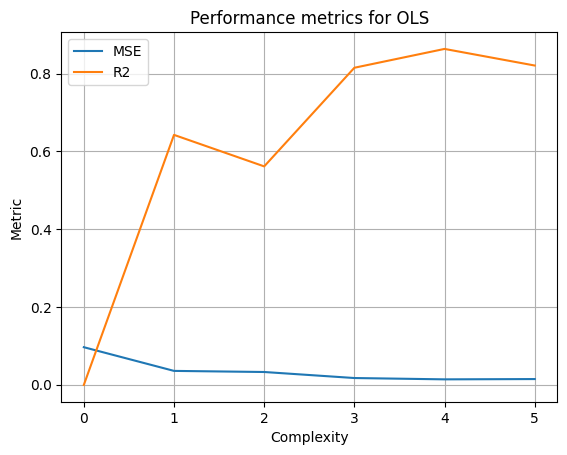
\includegraphics[width=0.5\linewidth]{Project_1/figures/OLS_MSE_R2.png}
    \caption{MSE- and R2-scores for OLS}
    \label{fig:MSE_R2_OLS}
\end{figure}

Fig.\ref{fig:MSE_R2_OLS} displays the MSE and $R^2$ values for OLS regression up to fifth degree polynomials. As we can see $R^2$ is optimal at complexity 4. Higher complexity does not affect the MSE significantly, which suggest that this is the optimal order when considering OLS. The drop in $R^2$ could suggest overfitting.

\begin{figure}[H]
    \centering
    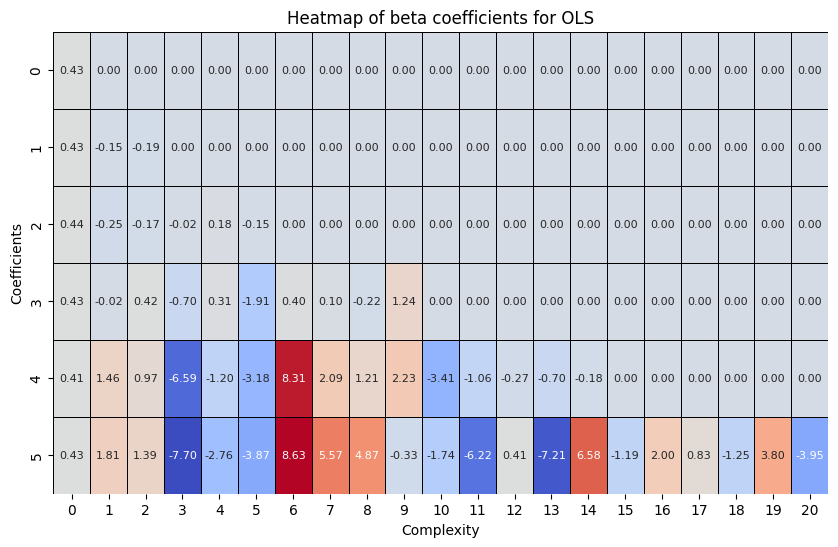
\includegraphics[width=0.9\linewidth]{Project_1/figures/beta_OLS.png}
    \caption{Beta coefficients for different polynomial complexity for OLS.}
    \label{fig:Beta_OLS}
\end{figure}

Fig.~\ref{fig:Beta_OLS} shows how the coefficients increase in magnitude when the order of the polynomial increases. As the magnitude increases we can get a better fit, but this can be at the cost of generalization.  

\subsubsection{Ridge}
\begin{figure}[H]
    \centering
    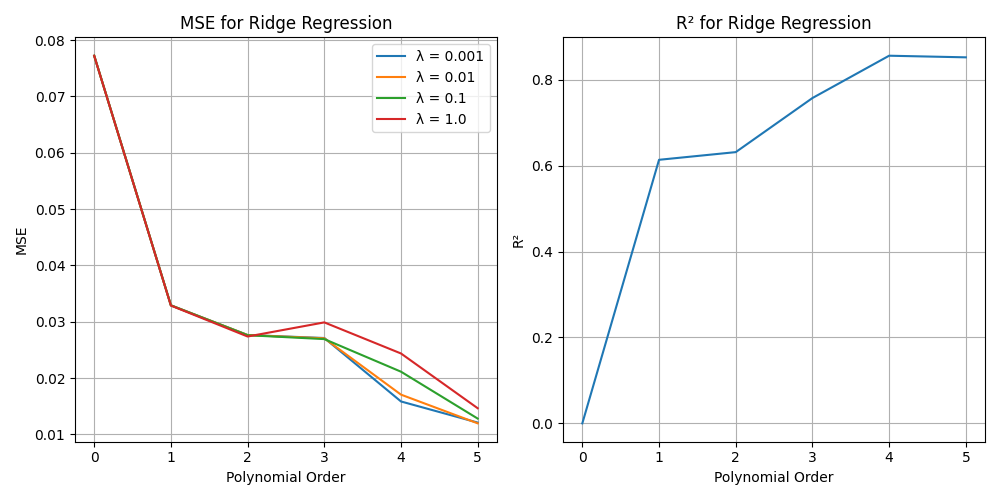
\includegraphics[width=0.9\linewidth]{Project_1/figures/ridge_mse_r2.png}
    \caption{Performance metrics for Ridge regression}
    \label{fig:ridge_mse_r2}
\end{figure}

In Fig.~\ref{fig:ridge_mse_r2} we see that the performance increases with lower values of $\lambda$. Contrast to OLS, we do not get a significant drop in $R^2$ for fifth order polynomials. This suggest that $p = 5$ and $\lambda = 0.001$ are the optimal parameters.

\subsubsection{Lasso}

\begin{figure}[H]
    \centering
    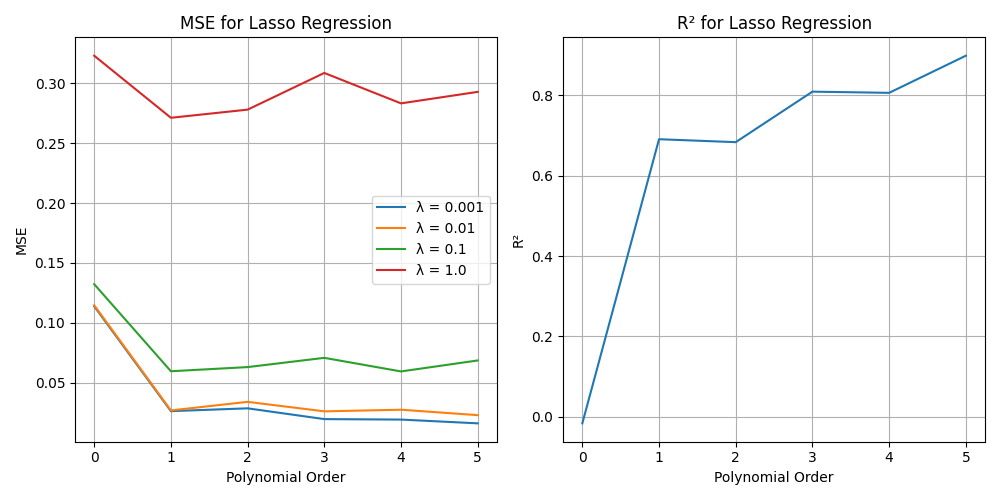
\includegraphics[width=0.9\linewidth]{Project_1/figures/lasso_mse_r2.png}
    \caption{Performance metrics for Lasso regression}
    \label{fig:lasso_mse_r2}
\end{figure}

In Fig.~\ref{fig:lasso_mse_r2} we again see that $\lambda = 0.001$ and $p = 5$ is optimal for the model.

\subsection{Bias-Variance trade-off}

\begin{figure}[H]
    \centering
    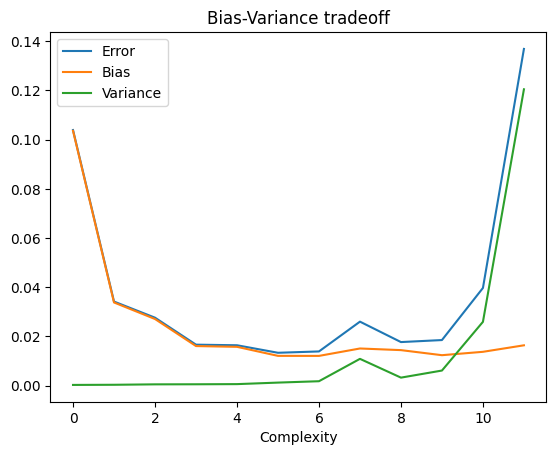
\includegraphics[width=0.9\linewidth]{Project_1/figures/Bias-Variance-Tradeoff-Bootstrap.png}
    \caption{Bias-Variance trade-off for OLS with bootstrap}
    \label{fig:bias_variance}
\end{figure}

Fig.~\ref{fig:bias_variance} shows that for low order polynomial fitting we have lower variance and higher bias and error. This corresponds to underfitting, as the model is not complex enough. As the complexity increases we get better results. But at around complexity 9-10 the variance increases drastically, which is due to overfitting.
 

\begin{figure}[H]
    \centering
    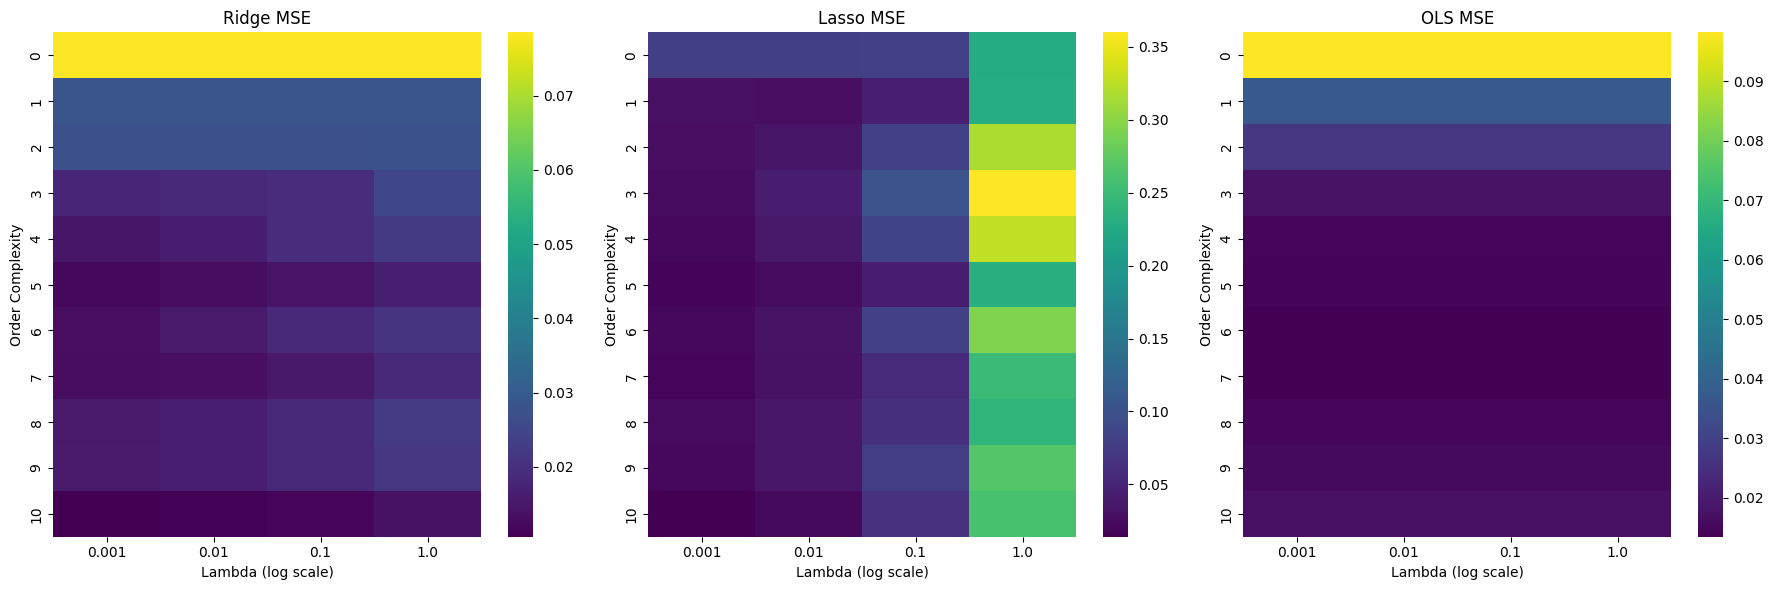
\includegraphics[width=1.0\linewidth]{Project_1/figures/Heatmap.png}
    \caption{Heatmap showing the MSE for each combination of order and lambda for the three regression models.}
    \label{fig:heatmap}
\end{figure}

In Fig.~\ref{fig:heatmap} we again find that increasing complexity and decreasing $\lambda$ yields better results.

\subsection{Terrain Data}

Moving on from the Franke function, we perform the same analysis for the provided terrain data. It is worth to note that due to the excessive size of the terrain data, we have for the sake of RAM and the environment decided to downsample the data to reduce dimensionality and hopefully noise, as well as trained the regression models on a random section of the downsampled image. The resulting image that will be used for training and future discussions are based on the terrain data of size (100, 100). 

\begin{figure}[H]
    \centering
    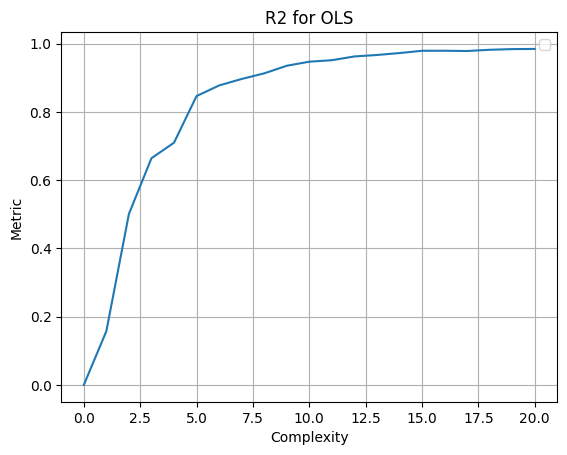
\includegraphics[width=0.6\linewidth]{Project_1/figures/R2_ols_terrain.png}
    \caption{R2 score for OLS on terrain data.}
    \label{fig:r2_terrain_ols}
\end{figure}

\begin{figure}[H]
    \centering
    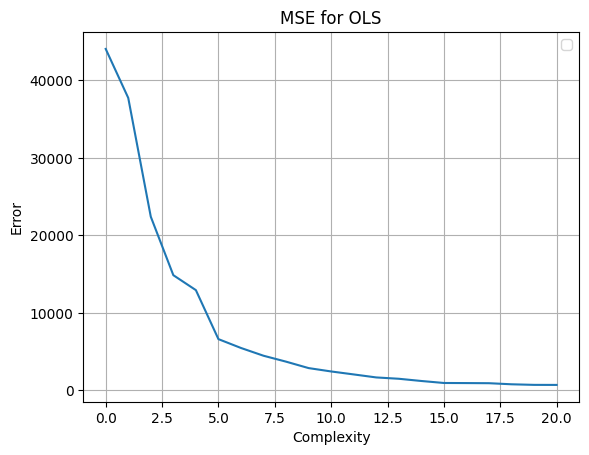
\includegraphics[width=0.6\linewidth]{Project_1/figures/mse_ols_terrain.png}
    \caption{MSE score for OLS on terrain data.}
    \label{fig:mse_terrain_ols}
\end{figure}

From FIG.~\ref{fig:r2_terrain_ols} and FIG.~\ref{fig:mse_terrain_ols} we can see that the OLS model is consistently performing better given the higher model complexity. This indicates that the model manages to fit the data better given the higher complexity.

\subsubsection{Ridge}
\begin{figure}[H]
    \centering
    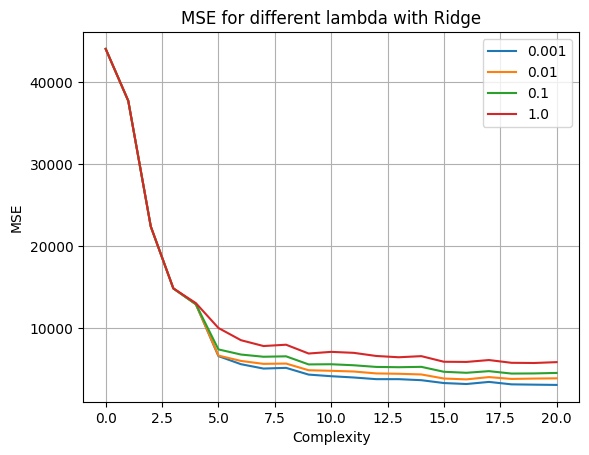
\includegraphics[width=0.6\linewidth]{Project_1/figures/MSE_ridge_terrain.png}
    \caption{MSE score for OLS with ridge regularization on terrain data.}
    \label{fig:mse_terrain_ridge}
\end{figure}

\subsubsection{Lasso}
\begin{figure}[H]
    \centering
    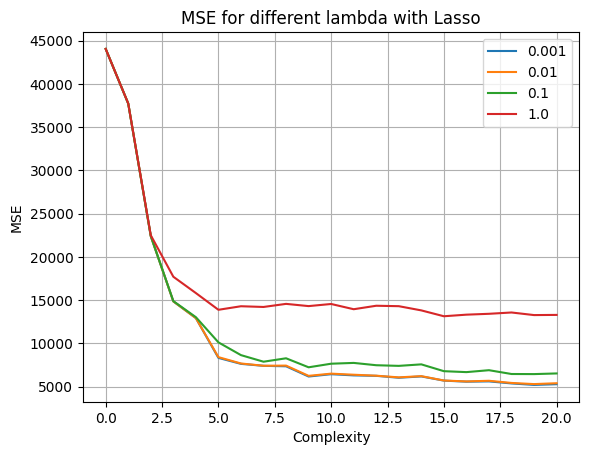
\includegraphics[width=0.6\linewidth]{Project_1/figures/MSE_lasso_terrain.png}
    \caption{MSE score for OLS with lasso regularization on terrain data.}
    \label{fig:mse_terrain_lasso}
\end{figure}

From FIG.~\ref{fig:mse_terrain_ridge} and FIG.~\ref{fig:mse_terrain_lasso} it can be observed that we get an increase in error the higher our $\lambda$ values are. Although the MSE values are higher for the lasso than the ridge. Indicating that ridge might be performing better than lasso.

\begin{figure}[H]
    \centering
    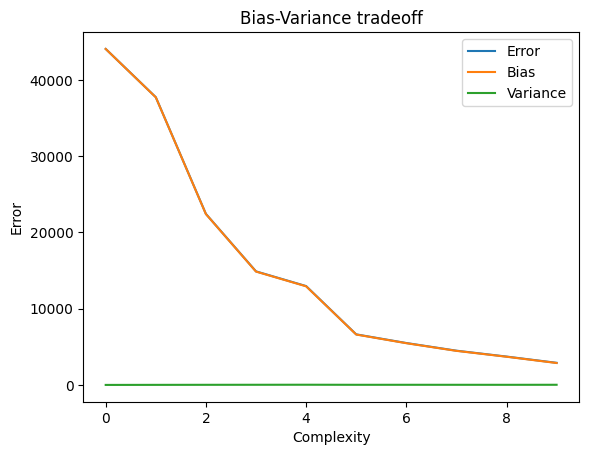
\includegraphics[width=0.6\linewidth]{Project_1/figures/Bias-Variance-Tradeoff-Bootstrap_Terrain.png}
    \caption{Bias variance tradeoff after performing bootstrap with 100 iterations.}
    \label{fig:bias-variance-terrain}
\end{figure}

From FIG.~\ref{fig:bias-variance-terrain} we can see that the error decreases as the model complexity increases. The same can be said for bias, while variance seems to remain low and constant throughout.

\begin{figure}[H]
    \centering
    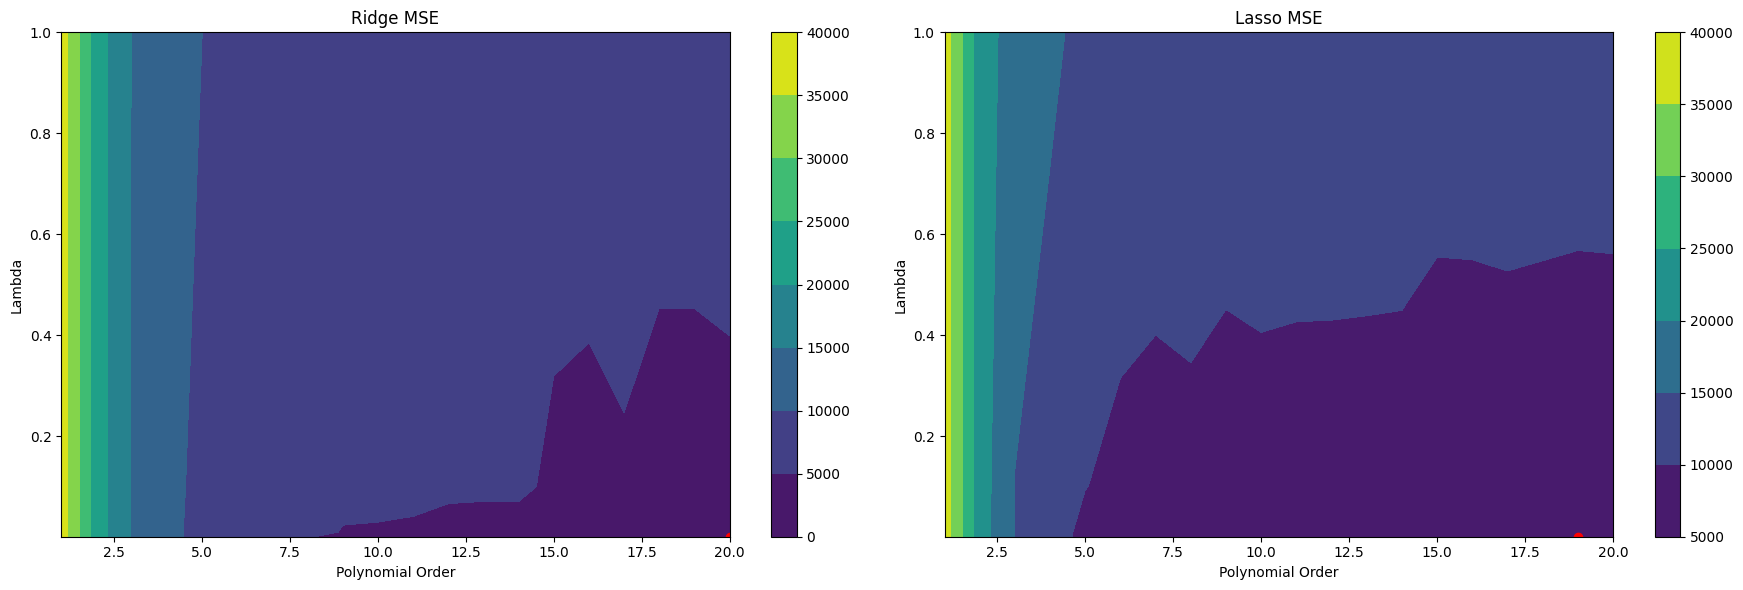
\includegraphics[width=0.9\linewidth]{Project_1/figures/countour_heatmap_mse.png}
    \caption{Countour}
    \label{fig:countour}
\end{figure}

From FIG.~\ref{fig:countour} we can see that the ridge regression seems to be performing better for lower values of $\lambda$ and higher complexity order. The same observation can be said for lasso, but the general error values seem to be of a higher degree, indicating that lasso regression is performing worse than ridge regression.

After performing k-fold cross-validation on all three regression models, we then find the lowest MSE value for all three across all $\lambda$ and polynomial orders.

\begin{algorithm\label{algo:scores}}
    min(MSE_{OLS}) = 2064 \\
    min(MSE_{ridge}) = 3152 \\
    min(MSE_{lasso}) = 7172 \\
\end{algorithm}

\section{Discussion}
\subsection{Regression Analysis of the Franke's Function}
\subsubsection{Discussion of Model Performance and the Differences of methods}
Comparing the different regression models from the test data, we can from the results see that OLS performs the best of minimising the MSE over Ridge and Lasso, where the latter has the highest score(worst)\ref{algo:scores}. The lower MSE-score for OLS suggests that it fits the terrain data more accurately, making fewer errors on average when predicting the data. A note on the MSE-score: a lower score diplays a better model performance as the models predicted valies are closer to the real data, producing fewer errors. For instance, in case with the terrain modeling we get a better representation of the terrain data and its complexity.

\subsubsection{Differences in the three models}

OLS tends to perform better when the data has lower variance in the estimates of the $\beta$-coefficients or when the model does not require regularization. In contrast, Ridge and Lasso apply regularization through the penalty-term $\lambda$ to prevent overfitting, which as we see from the perofmrance increase the MSE-score.


\subsubsection{Which model fits the data best?}
The MSE values for kfold ridge and kfold lasso seems to yield better results than kfold OLS when it comes to the fitting of Franke's function.

\subsubsection{ MSE in Kfold Cross-validation vs. MSE in Bootstrap}
Compare the MSE you get from your cross-validation code with the one you got from your bootstrap code. Comment your results. Try 5-10 folds.
In addition to using the ordinary least squares method, you should include
both Ridge and Lasso regression

Discuss the bias and variance trade-off as function of your model complexity
(the degree of the polynomial) and the number of data points, and possibly also
your training and test data using the bootstrap resampling method


\subsection{Terrain Data}
Initially, for the terrain data we used the whole data of the terrain to train and test our model. This proved to be a long run, considering that we also wanted to work with over 10 polynomials for better data representation in the plots. It took us time to understand how time consuming it can be to work on large volumes of data and this practice is far from beneficial. After this abuse, we pivoted towards using a reduced data set that consisted of 100x100 data points, which produced far quicker results. 

After comparing the three regression models, the evaluation of model performance based on the MSE across different complexities shows that OLS outperforms Ridge and Lasso in terms of fitting the data better with regards to MSE. This is rather surprising as Ridge and Lasso are designed to handle overfitting by adding regularization penalties to the loss function.

Some explanations to this could be that the terrain data had relatively low noise, and thus OLS may be sufficient to capture the underlying patterns without overfitting. In such cases, the penalties introduced by the regularizers could hinder performance. This would require some more exploratory data analysis of the terrain data to explore the level of noise in the data.

Furthermore, as we performed a k-fold cross-validation with up to a complexity order of 20, the OLS might have been complex enough to capture the data, but further validation in terms of overfitting has to be done to be sure. New unseen data should be used to validate the model performance.

We suspect that the unexpected results can stem from not scaling the z values of the terrain data, which had values ranging from 0 to 1800, but as this was our target data, we decided not to. Furthermore, the data that was used could potentially have been bigger, or more sections of the original data could have been used, which could give us a better representation of the model performances. An example could be to use a bigger section instead of a (100,100) patch.

\section{Conclusion and Further Work}

In this article we have explored and tested several regression methods and means of circumventing the difficulties involved with data, such as lack and imbalances.
Based on the results from testing different regression models on terrain data, OLS performs better than Ridge and Lasso in minimizing the MSE. This suggests that OLS fits the data more accurately, for our use case, likely due to the relatively low noise in the dataset, which reduces the need for regularization. While Ridge and Lasso are designed to prevent overfitting through the penalty-term $\lambda$, where in our use case, may have hindered performance. The results from the k-fold cross-validation indicates that OLS captured the terrain's complexity adequately, but further validation on unseen terrain data is necessary to confirm the model’s reliability in generalization to arbitrary terrain data.

\newpage

\section{Appendix}
\subsection{Analytical expression for the MSE \label{appendix:MSE}}
Assumptions:
\begin{enumerate}
    \item $\varepsilon \text{ is independent from } x \text{ which gives: }\mathbb{E}[\varepsilon]=0)$
    \item $y=f(x) + \varepsilon$ \text{. Here we will simplify f=f(x)}.
    \item $f(x) \text{ is a fixed, deterministic function of } x \text{, hence }\\ \mathbb{E}[f(x)]=f(x)$
\end{enumerate}
{The mean-square error of our model can be written:}
%
%_____________________________________
%
\begin{align*}
    & \text{MSE} = \mathbb{E}[(y-\Tilde{y})^2]\\
    & = \mathbb{E}[y^2-2y\Tilde{y}+\Tilde{y}^2]\\
    & = \mathbb{E}[y^2]-2\mathbb{E}[y\Tilde{y}]+\mathbb{E}[\Tilde{y}^2]\\
\end{align*}
%
We look into each term:
\begin{equation}
\mathbb{E}[y^2]
\end{equation}
\begin{equation}
    \mathbb{E}[y\Tilde{y}]
\end{equation}
\begin{equation}
    \mathbb{E}[\Tilde{y}^2]
\end{equation}
%
%Term 1 ____________
From (1) we have:
 \begin{align*}
     & \mathbb{E}[y^2]=\mathbb{E}[(f+\varepsilon)^2]=\mathbb{E}[f^2+2f\varepsilon+\epsilon^2]\\
     & = \mathbb{E}[f^2]+\mathbb{E}[\varepsilon^2]\\
     & =  \mathbb{E}[f^2]+\sigma^2 = f^2+\sigma^2
 \end{align*}
%Term 2 _________________
From (2):
\begin{align*}
    & \mathbb{E}[y\Tilde{y}]=\mathbb{E}[y]\mathbb{E}[\Tilde{y}]
     = \mathbb{E}[f+\varepsilon]\mathbb{E}[\Tilde{y}]\\
    & =\mathbb{E}[f]\mathbb{E}[\Tilde{y}]=f\mathbb{E}[\Tilde{y}]
\end{align*}
%Term 3 _________________
We have:
\begin{align*}
    & Var[\Tilde{y}]=\mathbb{E}[(\Tilde{y}]-\mathbb{E}[\Tilde{y}])^2]\\
    & = \mathbb{E}[\Tilde{y}^2-2\Tilde{y}\mathbb{E}[\Tilde{y}]+(\mathbb{E}[\Tilde{y}])^2]\\
    & = \mathbb{E}[\Tilde{y}^2]-2\mathbb{E}[\Tilde{y}]\mathbb{E}[\Tilde{y}]+(\mathbb{E}[\Tilde{y}])^2\\
    & = \mathbb{E}[\Tilde{y}^2]-(\mathbb{E}[\Tilde{y}])^2\\
    & \implies \mathbb{E}[\Tilde{y}^2]= Var[\Tilde{y}]+(\mathbb{E}[\Tilde{y}])^2
\end{align*}
%
Put the terms together:
\begin{align*}
    & \mathbb{E}[y^2]-2\mathbb{E}[y\Tilde{y}]+\mathbb{E}[\Tilde{y}^2]\\
    & = f^2+\sigma^2-2f\mathbb{E}[\Tilde{y}]+(Var(\Tilde{y})+(\mathbb{E}[\Tilde{y}])^2)\\
    & = f^2-2f\mathbb{E}[\Tilde{y}]+(\mathbb{E}[\Tilde{y}])^2+Var(\Tilde{y})+\sigma^2\\
    & \implies \mathbb{E}[(f-\mathbb{E}[\Tilde{y}])^2]+Var(\Tilde{y})+\sigma^2
\end{align*}

First term in above expression can be approximated:
\begin{equation}
    \mathbb{E}[(f-\mathbb{E}[\Tilde{y}])^2] \simeq \frac{1}{n}\sum_{i}(y_i-\mathbb{E}[\Tilde{y}])^2 \text{ ,where } f_i\simeq y_i
\end{equation}

From (4) we have that MSE can be written:
\begin{equation}
    \mathbb{E}[(f-\mathbb{E}[\Tilde{y}])^2] \simeq \frac{1}{n}\sum_{i}(y_i-\mathbb{E}[\Tilde{y}])^2 = Bias[\Tilde{y}]
\end{equation}

Similarly, the variance can be expressed as:
\begin{align*}
    \mathbb{E}[(\Tilde{y}-\mathbb{E}[\Tilde{y}])^2]\simeq\frac{1}{n}\sum_{i}(\Tilde{y_i}-\mathbb{E}[\Tilde{y}])^2 = Var[\Tilde{y}]
\end{align*}
%___________________________________________
Setting in both the bias and variance terms into the equation we obtain:

$MSE=Bias(\Tilde{y})+Var(\Tilde{y})+\sigma^2$
\hfill\break





\bibliographystyle{plain}
\bibliography{References} % add  references to this file
\end{document}